% ----------------------------------------------------------------------------
\section{Transport Protocols}
This chat protocol does not rely on a specific underlying transport protocol,
but is \textit{transport protocol independent}. 
Transport protocols are used to submit an onion to the next peer.

% -----------------------------------------------------------------------------
\subsection{Network packets ("`postcards"')}
\label{eofpostcard}
%Onions are encapsulated into the transport protocol specific
%packet type and sent out onto the network.
%The term Postcards are described in detail in chapter \ref{postcards}, page \pageref{postcards}.
A postcard "`packet"' contains one onion packet plus the transport protocol
shell. Postcard packets are the only packet type that is seen by a possible
attacker ("`on the wire"'). 
The name postcard was choosen to reflect the fact, that anyone
passing the postcard can read what is written on it.
% ----------------------------------------------------------------------------
\subsection{Tunneling}
\label{tunneling}
Due to the transport protocol independence, postcards can and should
be written into a variety of different transport protocol types.
This helps to circumvent firewall rules and blocking of a specific
traffic type. A lot of potential can be found in the reusage of
common protocols like HTTP and DNS.\cite{rfc1034, rfc1035, rfc2616}
The process is also called \textit{steganographic}.
% ----------------------------------------------------------------------------
\subsection{Multiplexing / Variable Addresses}
\label{multiplexing}
One peer should consider the availbility of itself via a variety
of addresses, so the chance of not being reachable is minimised.
Figure \ref{addressmultiplexing} shows an example list of addresses
a peer could be reachable.
\begin{figure}
    \centering
    \caption{Adress Multiplexing}
    \label{addressmultiplexing}
    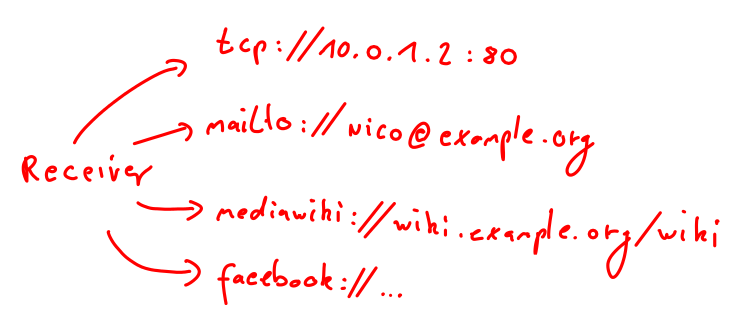
\includegraphics[scale=0.8]{addressmultiplexing.png}
\end{figure}
Theis multiplexing of addresses allows different transports to be used
for one peer, so that there is a higher diversity in outgoing packets.
% ----------------------------------------------------------------------------
\subsection{Access Methods}
\label{accessmethods}
Transport protocols can either be accessable \textit{directly} or 
\textit{indirectly}. In case of direct access (figure \ref{directaccess})
the sending peer directly connects to the receiving peer.
\begin{figure}
    \centering
    \caption{Direct Access}
    \label{directaccess}
    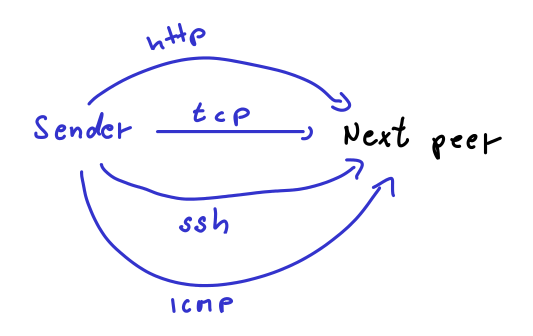
\includegraphics[scale=0.8]{directaccess.png}
\end{figure}
In case of indirect access, the sender stores the postcard on a intermediate
server and the receiving peer polls this server for postcards, as shown
in figure \ref{indirectaccess}.
\begin{figure}
    \centering
    \caption{Indirect Access}
    \label{indirectaccess}
    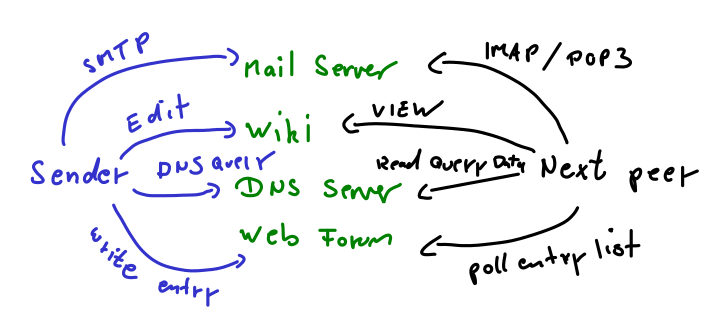
\includegraphics[scale=0.8]{indirectaccess.png}
\end{figure}
% ----------------------------------------------------------------------------
\subsection{List of Supported Transports}
To ensure interoperability, clients which support a specific
protocol version must support all listed transport protocols. This version
supports all protocols specified in table \ref{transportprotocollisting}.
\begin{longtable}{|c|c|c|}
\caption{Transport protocols}
\label{transportprotocollisting}
\\
\hline
\textbf{Protocol} & \textbf{Description} & \textbf{Supported versions}\\
\hline
tcp & Transmission Control Protocol & 0.1 - 0.1\\
\hline
\end{longtable}
